\section{Sample selection}
\label{sec:sample}

We searched \NWindows{} spectral windows toward \NStars{} stars in
\NSystems{} independent systems within 40\,pc, drawn from \NEB{} public
ALMA execution blocks and \TotalDataTB\,TB of raw data through one frozen
pipeline. The sample is two experiments, not one. \NWinA{} windows toward
\NSysClassA{} systems are fine-channel, called \emph{Class~A} throughout:
these resolve a drifting carrier and are the primary experiment, and
every sensitivity and every exclusion quoted in this paper refers to them
unless stated otherwise. The remaining \NWinB{} windows are
coarse-channel, \emph{Class~B}, and support a secondary search for
unresolved spectral excess; they can register a spike but cannot
distinguish a drifting signal from a stationary one. Table
\ref{tab:searchspace} collects the survey as searched.

The inclusion criteria are objective and were applied by query. A star
enters if its Gaia~DR3 parallax is at least 25\,mas, measured to better
than \PlxAdqlPct{} per cent. It must also have its proper-motion-corrected
position at the observation epoch inside the quoted field of view of at
least one public ALMA execution block. Distances are direct inversions,
$d=1/\varpi$. The star need not sit at the pointing centre. Disc, planet
and spectral type enter as descriptive metadata only, and no star or
window was excluded by an unlisted criterion or for short integration.
The query returns \NCensus{} work-list entries; the quoted field of view
is optimistic, and only \NGenuinelyCovered{} of those stars are in fact
contained by a public field, of which \NStars{} yielded a searchable
window (Fig.~\ref{fig:funnel}). The complete per-star and per-window
ledger, including the five-criterion decision tree and every edge case,
is in the data release.

\subsection{The archival selection}
\label{sec:bias}

This sample was not designed. It is whatever previous ALMA programmes
happened to observe, for their own reasons, and
\PctDiscProposal{} per cent of the stars searched were targeted under a
debris-disc or planet-formation proposal. The consequence is a strong and
measurable bias, tabulated against a volume-limited reference census in
Table~\ref{tab:selfunc}: the sample is enriched in F and G stars and
depleted in M~dwarfs. Only \NMSearched{} of the \NMCensus{} catalogued
M~dwarfs within 40\,pc appear in it at all, and only \NClassAM{} have
Class~A coverage, the only coverage that can resolve a drifting carrier. Coverage is also concentrated: \ConcThreeWin{} of the
\NWindows{} windows come from \ConcThreeSys{} systems. Every statistical
statement in this paper is therefore a statement about an
archive-selected sample of nearby stars. None of them is an occurrence
rate for the solar neighbourhood, and because M~dwarfs host most of the
nearby habitable-zone planets, this survey cannot constrain transmitters
around the kind of star most likely to have one. The systems a targeted
search would itself have chosen are collected in
Table~\ref{tab:interesting}.

% Generated by make_tables_v328.py -- do not edit by hand.
\begin{table}
\centering
\scriptsize
\setlength{\tabcolsep}{4pt}
\caption{Selection function of the searched sample against a volume-limited reference census: Gaia~DR3 sources with $\varpi>0$, $\sigma_\varpi/\varpi\le0.1$ and $1/\varpi\le40$\,pc (17566 objects, of which 8594 carry a \texttt{teff\_gspphot} estimate, 49 per cent), against the 89 stars with at least one searched window. Temperatures are available for 53 of the 89 (all 89 matched to the 168-entry ALMA-covered census, 56 by exact name; 53 of those matches carry a temperature), so the temperature panel is normalised over classified objects only. ``Ratio'' is the sample column fraction over the census column fraction; $>1$ is over-representation.}
\label{tab:selfunc}
\begin{tabular}{@{}lrrr@{}}
\toprule
Property & Census & Searched & Ratio \\
\midrule
\multicolumn{4}{@{}l}{Distance (all 89 searched stars; 17566 census objects)} \\
\quad $d\le5$\,pc & 48 (0.3\%) & 12 (13.5\%) & 49.3 \\
\quad 5--10\,pc & 240 (1.4\%) & 13 (14.6\%) & 10.7 \\
\quad 10--20\,pc & 2069 (11.8\%) & 18 (20.2\%) & 1.7 \\
\quad 20--30\,pc & 5391 (30.7\%) & 19 (21.3\%) & 0.7 \\
\quad 30--40\,pc & 9818 (55.9\%) & 27 (30.3\%) & 0.5 \\
\midrule
\multicolumn{4}{@{}l}{$T_{\rm eff}$ class$^{a}$ (53 searched; 8594 census)} \\
\quad A ($\ge7500$\,K) & 24 (0.3\%) & 1 (1.9\%) & 6.8 \\
\quad F (6000--7500\,K) & 402 (4.7\%) & 9 (17.0\%) & 3.6 \\
\quad G (5300--6000\,K) & 860 (10.0\%) & 16 (30.2\%) & 3.0 \\
\quad K (3900--5300\,K) & 1400 (16.3\%) & 6 (11.3\%) & 0.7 \\
\quad M ($<3900$\,K) & 5908 (68.7\%) & 21 (39.6\%) & 0.6 \\
\midrule
\multicolumn{4}{@{}l}{Other axes} \\
\quad Known planet hosts$^{b}$ & 20 (11.9\%) & 23 (25.8\%) & 2.2 \\
\quad Searched stars / systems & -- & 89 / 82 & -- \\
\bottomrule
\end{tabular}

\smallskip
{\footnotesize $^{a}$Bins are temperature bins, not MK types: A $\ge7500$, F 6000--7500, G 5300--6000, K 3900--5300, M $<3900$\,K. Gaia \texttt{teff\_gspphot} is unavailable for about half the reference census, preferentially for the coolest and faintest objects, so the census M fraction is a lower limit and the earlier-type ratios are correspondingly upper limits. White dwarfs are not separable in this parameterisation and fall wherever their (unreliable) photometric temperature places them.\\ $^{b}$The Gaia reference census carries no planet information; the census column here is instead the 168-entry ALMA-covered census, of which 20 entries are known planet hosts. The 89 searched stars include 23 hosts of 50 known planets.}
\end{table}


\begin{figure} \centering
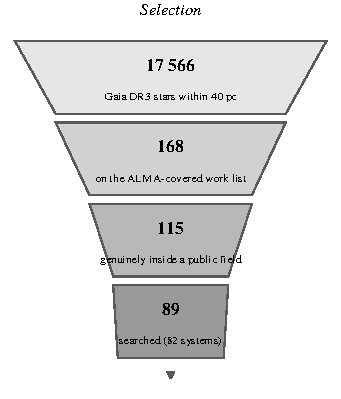
\includegraphics[width=0.66\columnwidth]{figures/selection_funnel.pdf}
\caption{The selection funnel, from the catalogued population within
40\,pc to the stars with a searched window. The three quantities the text
keeps apart are the \NCensus-entry work list the archive query returns,
the \NGenuinelyCovered{} stars a public field genuinely contains, and the
\NStars{} that yielded a searchable window. The chain applied to what
comes out of the funnel is Fig.~\ref{fig:chain}.}
\label{fig:funnel}
\end{figure}

\subsection{Frequency coverage and archival scope}
\label{sec:coverage}

The Class~A experiment covers $\Delta\nu_A=\DnuA$\,GHz of unique sky
frequency, and that coverage is sparse: it is \DomAIslands{} disjoint
islands scattered between \DomAFreqLo{} and \DomAFreqHi\,GHz, not a
band. The endpoints are a range over which observations exist, never a
range that was covered. Adding the coarse-channel windows brings the
total archival coverage to \DnuAB\,GHz in \UnionIntervals{} intervals, of
which \SearchedUnionGHz\,GHz survives the molecular-line mask of
\S\ref{sec:method}. The distribution is shown in
Fig.~\ref{fig:waterfall}; a transmitter at a frequency between the
islands was never observable here, whatever its power.

\begin{figure*}
\centering
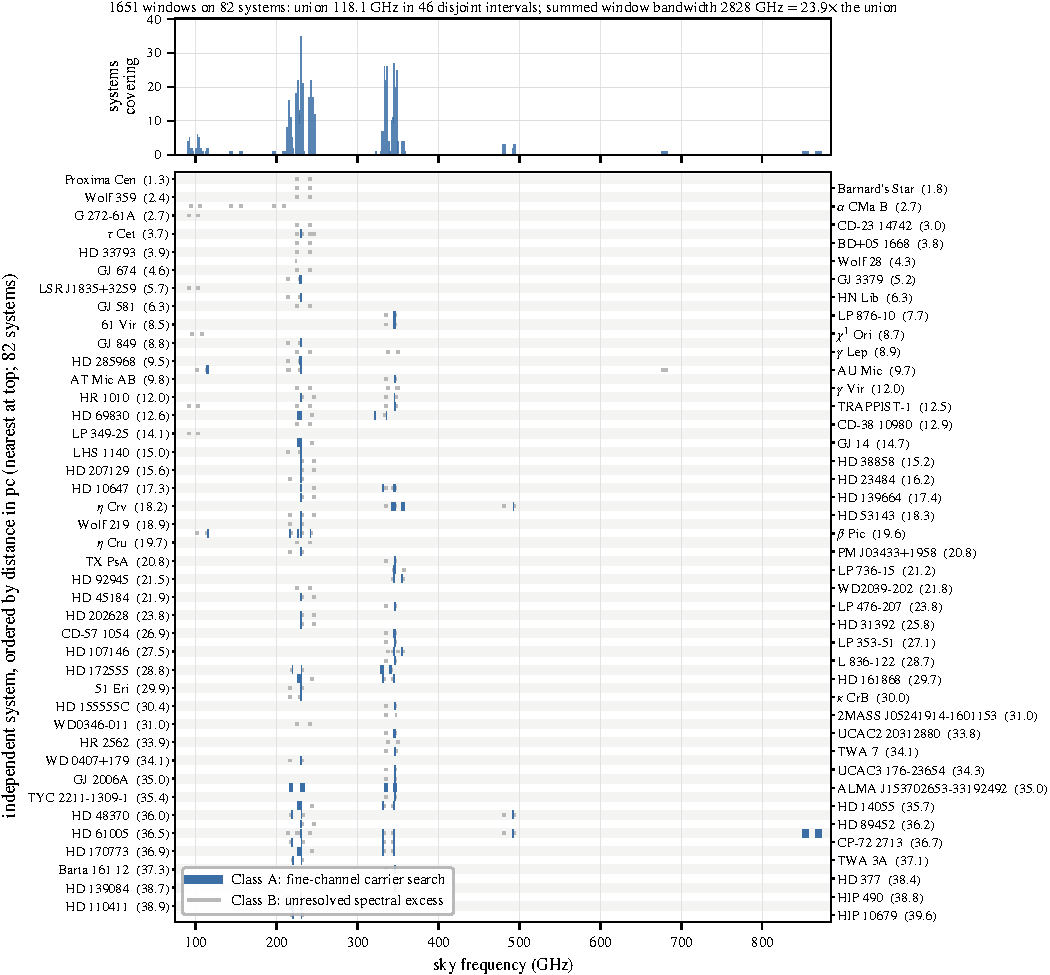
\includegraphics[width=0.99\textwidth]{figures/coverage_waterfall.pdf}
\caption{Where this survey searched. \emph{Lower panel:} each searched
window is a horizontal segment on its host system's row, rows ordered by
distance and labelled alternately on the left and right axes; heavy blue
marks the fine-channel carrier search (Class~A) and light grey the
coarse-channel spectral-excess search (Class~B). \emph{Upper panel:} the number
of systems covering each gigahertz of sky frequency; the threshold
distribution is Fig.~\ref{fig:context}(a). The coverage is narrow, clustered
and repeatedly revisited: \UnionIntervals{} islands concentrated near 230
and 345\,GHz, with summed window bandwidth $\GrossOverUnion\times$ the
union. The union measures frequency coverage, the summed bandwidth
integrated search effort.}
\label{fig:waterfall}
\end{figure*}

Of the \FateScope{} execution blocks in scope for this search,
\FateDone{} were calibrated and searched. The shortfall is accounted for
rather than estimated. For \FateNoCal{} blocks, \FateNoCalGB\,GB in all,
the archive holds only raw visibilities that were never
pipeline-calibrated; this is the single largest gap, and no effort on our
side would close it. A further \FateCalFail{} blocks failed calibration,
\FateUnattempted{} were not attempted, and \FateInfeas{} needed more
working disk than was available.

\begin{table}
\centering
\scriptsize
\caption{Systems of particular interest: every sample system within
15\,pc hosting at least one confirmed planet, ordered by distance.
$N_{\rm pl}$ is the confirmed-planet count, $N_{\rm A}$ the number of
Class~A windows, EIRP$_{90}$ the deepest Class~A sensitivity reached, and
$N_{\rm eb}$ the number of execution blocks covering the system, so
$N_{\rm eb}>1$ means repeat epochs exist. Six of these systems have no
Class~A coverage and so carry no drift-resolving limit --- the archival
selection of \S\ref{sec:bias} acting on exactly the targets a
transmitter search would choose. The full target list is in the data
release.}
\label{tab:interesting}
%% GENERATED by mk_interesting.py -- do not hand-edit.
\begin{tabular}{@{}l@{~~}r@{~~}r@{~~}l@{~~}r@{~~}r@{~~}r@{}}
\hline
System & $d$ & $N_{\rm pl}$ & Bands & $N_{\rm A}$ & EIRP$_{90}$ & $N_{\rm eb}$ \\
 & (pc) & & & & (W) & \\
\hline
Proxima Cen & 1.3 & 2 & 6 & 0 & -- & 25 \\
Barnard's Star & 1.8 & 4 & 6 & 0 & -- & 3 \\
$\tau$~Cet & 3.7 & 3 & 6 & 6 & $1.7\times10^{14}$ & 8 \\
BD+05 1668 (GJ 273) & 3.8 & 2 & 6 & 0 & -- & 25 \\
HD 33793 & 3.9 & 1 & 6 & 0 & -- & 22 \\
GJ 674 & 4.6 & 1 & 6 & 0 & -- & 20 \\
HN Lib & 6.3 & 1 & 6 & 5 & $5.6\times10^{14}$ & 5 \\
GJ 581 & 6.3 & 3 & 6 & 0 & -- & 9 \\
61 Vir & 8.5 & 3 & 7 & 5 & $1.8\times10^{14}$ & 5 \\
GJ 849 & 8.8 & 2 & 6 & 6 & $9.9\times10^{14}$ & 6 \\
HD 285968 & 9.5 & 1 & 6 & 4 & $1.3\times10^{15}$ & 4 \\
AU Mic & 9.7 & 4 & 3,6,9 & 13 & $1.7\times10^{14}$ & 14 \\
TRAPPIST$-$1 & 12.5 & 7 & 3,6,7 & 5 & $2.4\times10^{14}$ & 18 \\
HD 69830 & 12.6 & 3 & 6,7 & 22 & $1.7\times10^{14}$ & 8 \\
LHS 1140 & 15.0 & 2 & 6 & 4 & $2.8\times10^{15}$ & 4 \\
\hline
\end{tabular}

\end{table}

\begin{table}
\centering
\scriptsize
\caption{The survey as searched. Every frequency union quoted here is an
aggregate over clustered, repeatedly revisited coverage, whose
distribution is Fig.~\ref{fig:waterfall}; no union should be read as
continuous coverage between its endpoints. Powers and frequencies are
given to two significant figures, except where a channel or sky frequency
must be matched to the released catalogue and is given to the precision
the grid supports.}
\label{tab:searchspace}
\begin{tabular}{@{}P{0.53\columnwidth}P{0.40\columnwidth}@{}}
\hline
Quantity & Value \\
\hline
Stars searched; independent systems & \NStars{}; \NSystems{} \\
\quad work-list entries; genuinely covered & \NCensus{};
\NGenuinelyCovered{} \\
Execution blocks; distance range & \NEB{}; \DistMin--\DistMax\,pc \\
Spectral windows searched & \NWindows{} \\
\quad Class~A fine / Class~B coarse & \NWinA{} / \NWinB{}
(\PctCoarse\% Class~B) \\
\quad 12\,m array; ACA 7\,m & \NWinTwelveM{}; \NWinSevenM{} \\
Native channel widths & 15.3\,kHz--31.25\,MHz; median
\ChanMedianMHz\,MHz \\
\emph{$\Delta\nu_A$, unique Class~A frequency union} (the
drifting-carrier experiment) & $\mathbf{\DnuA}$\,GHz in
\DomAIslands{} islands, \DomAFreqLo--\DomAFreqHi\,GHz \\
\quad coverage Class~B adds & \DnuBonly\,GHz \\
\quad total archival coverage & \DnuAB\,GHz (\UnionIntervals{} intervals)
\\
\quad usable after the molecular-line mask & \SearchedUnionGHz\,GHz \\
Nominal trigger $P_{\rm trig}$, Class~A; Class~B &
$\EirpMinA$--$\EirpMaxA$\,W; $\EirpMinB$--$\EirpMaxB$\,W \\
Execution blocks in scope; searched & \FateScope{}; \FateDone{} \\
\hline
\end{tabular}
\end{table}

%% REQUEST (stack-discussion owner, sections/06_discussion.tex): your R3(d)
%% is settled here. The block ledger's headline (\FateScope, \FateDone,
%% \FateNoCal, \FateCalFail, \FateUnattempted, \FateInfeas) is now two
%% sentences in \S\ref{sec:sample}, because it is a stated limitation and a
%% stated limitation may not live only in the data release. Please cite
%% \S\ref{sec:sample} and do not restate the counts. Your R1 is also
%% settled: sec:bias is defined above.
%% REQUEST (numbers owner): tab_interesting.tex is generated by
%% referee_r9/sample/mk_interesting.py, which reads the released
%% catalogue, the frozen census, the confirmed-planet table and
%% \SelRatioRank out of the macro layer. It has eight assertions and five
%% drives. Please adopt it into make_all.sh so the table regenerates with
%% everything else. Two display defects in it are yours, not mine: the
%% catalogue designation of Barnard's Star prints as a SIMBAD identifier
%% with the "NAME" prefix stripped, and BD+05 1668 would read better with
%% its GJ alias beside it. Both belong in star_alias.designation.
%% REQUEST (numbers owner): the sensitivity rows have been removed from
%% Table~\ref{tab:searchspace} rather than restated, because the
%% multiplier they were computed on is not the one this paper adopts. When
%% \EirpNinetyMultA and \EirpNinetyMultB exist, the fine- and
%% coarse-channel EIRP$_{90}$ ranges should return to this table as two
%% rows, per window and per system.
%% REQUEST (method owner, sections/04_method.tex): \S\ref{sec:summary}
%% duplicates part of Table~\ref{tab:searchspace}. One of the two should
%% carry the survey summary; this table is the shorter.
